\section{Ellipse Class Reference}
\label{classEllipse}\index{Ellipse@{Ellipse}}
{\tt \#include $<$ellipse.h$>$}

Inheritance diagram for Ellipse::\begin{figure}[H]
\begin{center}
\leavevmode
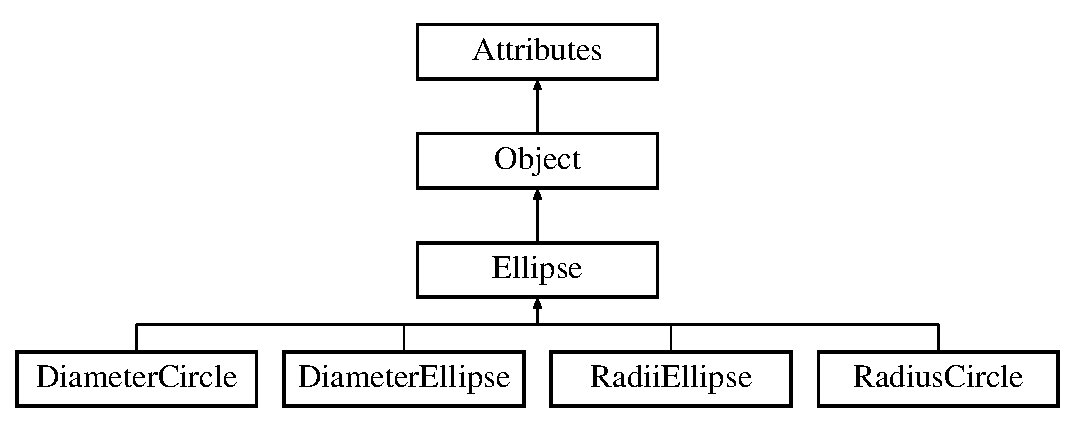
\includegraphics[height=4cm]{classEllipse}
\end{center}
\end{figure}
\subsection*{Public Methods}
\begin{CompactItemize}
\item 
{\bf Ellipse} ()
\item 
{\bf $\sim$Ellipse} ()
\item 
int {\bf get\-Sub\-Type} ()
\item 
void {\bf set\-Angle} (float {\bf angle})
\item 
float {\bf get\-Angle} ()
\item 
void {\bf set\-Center} ({\bf Coordinate} $\ast${\bf center})
\item 
{\bf Coordinate} $\ast$ {\bf get\-Center} ()
\item 
void {\bf set\-Radii} ({\bf Coordinate} $\ast${\bf radius})
\item 
{\bf Coordinate} $\ast$ {\bf get\-Radii} ()
\item 
void {\bf set\-Start} ({\bf Coordinate} $\ast${\bf start})
\item 
{\bf Coordinate} $\ast$ {\bf get\-Start} ()
\item 
void {\bf set\-End} ({\bf Coordinate} $\ast${\bf end})
\item 
{\bf Coordinate} $\ast$ {\bf get\-End} ()
\item 
void {\bf write} (std::ostream \&stream) const
\end{CompactItemize}
\subsection*{Protected Methods}
\begin{CompactItemize}
\item 
void {\bf set\-Sub\-Type} (int {\bf sub\-Type})
\end{CompactItemize}
\subsection*{Protected Attributes}
\begin{CompactItemize}
\item 
int {\bf sub\-Type}
\item 
int {\bf direction}
\item 
float {\bf angle}
\item 
{\bf Coordinate} $\ast$ {\bf center}
\item 
{\bf Coordinate} $\ast$ {\bf radii}
\item 
{\bf Coordinate} $\ast$ {\bf start}
\item 
{\bf Coordinate} $\ast$ {\bf end}
\end{CompactItemize}


\subsection{Detailed Description}
This class handles ellipses and circles. This class is derived from {\bf Object} {\rm (p.\,\pageref{classObject})}. \begin{Desc}
\item[Author: ]\par
Anthony Liekens \end{Desc}




\subsection{Constructor \& Destructor Documentation}
\index{Ellipse@{Ellipse}!Ellipse@{Ellipse}}
\index{Ellipse@{Ellipse}!Ellipse@{Ellipse}}
\subsubsection{\setlength{\rightskip}{0pt plus 5cm}Ellipse::Ellipse ()}\label{classEllipse_a0}


\index{Ellipse@{Ellipse}!~Ellipse@{$\sim$Ellipse}}
\index{~Ellipse@{$\sim$Ellipse}!Ellipse@{Ellipse}}
\subsubsection{\setlength{\rightskip}{0pt plus 5cm}Ellipse::$\sim$Ellipse ()}\label{classEllipse_a1}




\subsection{Member Function Documentation}
\index{Ellipse@{Ellipse}!getAngle@{getAngle}}
\index{getAngle@{getAngle}!Ellipse@{Ellipse}}
\subsubsection{\setlength{\rightskip}{0pt plus 5cm}float Ellipse::get\-Angle ()\hspace{0.3cm}{\tt  [inline]}}\label{classEllipse_a4}


Returns the angle. \begin{Desc}
\item[Returns: ]\par
float \end{Desc}


Reimplemented from {\bf Attributes} {\rm (p.\,\pageref{classAttributes_a39})}.\index{Ellipse@{Ellipse}!getCenter@{getCenter}}
\index{getCenter@{getCenter}!Ellipse@{Ellipse}}
\subsubsection{\setlength{\rightskip}{0pt plus 5cm}{\bf Coordinate}$\ast$ Ellipse::get\-Center ()\hspace{0.3cm}{\tt  [inline]}}\label{classEllipse_a6}


\index{Ellipse@{Ellipse}!getEnd@{getEnd}}
\index{getEnd@{getEnd}!Ellipse@{Ellipse}}
\subsubsection{\setlength{\rightskip}{0pt plus 5cm}{\bf Coordinate}$\ast$ Ellipse::get\-End ()\hspace{0.3cm}{\tt  [inline]}}\label{classEllipse_a12}


\index{Ellipse@{Ellipse}!getRadii@{getRadii}}
\index{getRadii@{getRadii}!Ellipse@{Ellipse}}
\subsubsection{\setlength{\rightskip}{0pt plus 5cm}{\bf Coordinate}$\ast$ Ellipse::get\-Radii ()\hspace{0.3cm}{\tt  [inline]}}\label{classEllipse_a8}


\index{Ellipse@{Ellipse}!getStart@{getStart}}
\index{getStart@{getStart}!Ellipse@{Ellipse}}
\subsubsection{\setlength{\rightskip}{0pt plus 5cm}{\bf Coordinate}$\ast$ Ellipse::get\-Start ()\hspace{0.3cm}{\tt  [inline]}}\label{classEllipse_a10}


\index{Ellipse@{Ellipse}!getSubType@{getSubType}}
\index{getSubType@{getSubType}!Ellipse@{Ellipse}}
\subsubsection{\setlength{\rightskip}{0pt plus 5cm}int Ellipse::get\-Sub\-Type ()\hspace{0.3cm}{\tt  [inline]}}\label{classEllipse_a2}


\index{Ellipse@{Ellipse}!setAngle@{setAngle}}
\index{setAngle@{setAngle}!Ellipse@{Ellipse}}
\subsubsection{\setlength{\rightskip}{0pt plus 5cm}void Ellipse::set\-Angle (float {\em angle})\hspace{0.3cm}{\tt  [inline]}}\label{classEllipse_a3}


Set the angle. \begin{Desc}
\item[Parameters: ]\par
\begin{description}
\item[{\em 
angle}]float value \end{description}
\end{Desc}
\begin{Desc}
\item[Returns: ]\par
void \end{Desc}


Reimplemented from {\bf Attributes} {\rm (p.\,\pageref{classAttributes_a17})}.\index{Ellipse@{Ellipse}!setCenter@{setCenter}}
\index{setCenter@{setCenter}!Ellipse@{Ellipse}}
\subsubsection{\setlength{\rightskip}{0pt plus 5cm}void Ellipse::set\-Center ({\bf Coordinate} $\ast$ {\em center})\hspace{0.3cm}{\tt  [inline]}}\label{classEllipse_a5}


\index{Ellipse@{Ellipse}!setEnd@{setEnd}}
\index{setEnd@{setEnd}!Ellipse@{Ellipse}}
\subsubsection{\setlength{\rightskip}{0pt plus 5cm}void Ellipse::set\-End ({\bf Coordinate} $\ast$ {\em end})\hspace{0.3cm}{\tt  [inline]}}\label{classEllipse_a11}


\index{Ellipse@{Ellipse}!setRadii@{setRadii}}
\index{setRadii@{setRadii}!Ellipse@{Ellipse}}
\subsubsection{\setlength{\rightskip}{0pt plus 5cm}void Ellipse::set\-Radii ({\bf Coordinate} $\ast$ {\em radius})\hspace{0.3cm}{\tt  [inline]}}\label{classEllipse_a7}


\index{Ellipse@{Ellipse}!setStart@{setStart}}
\index{setStart@{setStart}!Ellipse@{Ellipse}}
\subsubsection{\setlength{\rightskip}{0pt plus 5cm}void Ellipse::set\-Start ({\bf Coordinate} $\ast$ {\em start})\hspace{0.3cm}{\tt  [inline]}}\label{classEllipse_a9}


\index{Ellipse@{Ellipse}!setSubType@{setSubType}}
\index{setSubType@{setSubType}!Ellipse@{Ellipse}}
\subsubsection{\setlength{\rightskip}{0pt plus 5cm}void Ellipse::set\-Sub\-Type (int {\em sub\-Type})\hspace{0.3cm}{\tt  [inline, protected]}}\label{classEllipse_b0}


\index{Ellipse@{Ellipse}!write@{write}}
\index{write@{write}!Ellipse@{Ellipse}}
\subsubsection{\setlength{\rightskip}{0pt plus 5cm}void Ellipse::write (std::ostream \& {\em stream}) const\hspace{0.3cm}{\tt  [virtual]}}\label{classEllipse_a13}


Write the object to a given outstream. All inherited classes of object should provide this method, since it's called by {\bf Figure} {\rm (p.\,\pageref{classFigure})} (the object container) to output objects to a given stream. \begin{Desc}
\item[Parameters: ]\par
\begin{description}
\item[{\em 
stream}]output stream \end{description}
\end{Desc}
\begin{Desc}
\item[Returns: ]\par
void \end{Desc}


Reimplemented from {\bf Object} {\rm (p.\,\pageref{classObject_a3})}.

\subsection{Member Data Documentation}
\index{Ellipse@{Ellipse}!angle@{angle}}
\index{angle@{angle}!Ellipse@{Ellipse}}
\subsubsection{\setlength{\rightskip}{0pt plus 5cm}float Ellipse::angle\hspace{0.3cm}{\tt  [protected]}}\label{classEllipse_n2}




Reimplemented from {\bf Attributes} {\rm (p.\,\pageref{classAttributes_n13})}.\index{Ellipse@{Ellipse}!center@{center}}
\index{center@{center}!Ellipse@{Ellipse}}
\subsubsection{\setlength{\rightskip}{0pt plus 5cm}{\bf Coordinate}$\ast$ Ellipse::center\hspace{0.3cm}{\tt  [protected]}}\label{classEllipse_n3}


\index{Ellipse@{Ellipse}!direction@{direction}}
\index{direction@{direction}!Ellipse@{Ellipse}}
\subsubsection{\setlength{\rightskip}{0pt plus 5cm}int Ellipse::direction\hspace{0.3cm}{\tt  [protected]}}\label{classEllipse_n1}


\index{Ellipse@{Ellipse}!end@{end}}
\index{end@{end}!Ellipse@{Ellipse}}
\subsubsection{\setlength{\rightskip}{0pt plus 5cm}{\bf Coordinate} $\ast$ Ellipse::end\hspace{0.3cm}{\tt  [protected]}}\label{classEllipse_n6}


\index{Ellipse@{Ellipse}!radii@{radii}}
\index{radii@{radii}!Ellipse@{Ellipse}}
\subsubsection{\setlength{\rightskip}{0pt plus 5cm}{\bf Coordinate}$\ast$ Ellipse::radii\hspace{0.3cm}{\tt  [protected]}}\label{classEllipse_n4}


\index{Ellipse@{Ellipse}!start@{start}}
\index{start@{start}!Ellipse@{Ellipse}}
\subsubsection{\setlength{\rightskip}{0pt plus 5cm}{\bf Coordinate}$\ast$ Ellipse::start\hspace{0.3cm}{\tt  [protected]}}\label{classEllipse_n5}


\index{Ellipse@{Ellipse}!subType@{subType}}
\index{subType@{subType}!Ellipse@{Ellipse}}
\subsubsection{\setlength{\rightskip}{0pt plus 5cm}int Ellipse::sub\-Type\hspace{0.3cm}{\tt  [protected]}}\label{classEllipse_n0}




The documentation for this class was generated from the following files:\begin{CompactItemize}
\item 
{\bf ellipse.h}\item 
{\bf ellipse.cpp}\end{CompactItemize}
